% 29 May 2001 
%	comments from Chris
% 30 May 2001 with comments from Fred
% 30 May 2001 with comments from Paola
% 30 May 2001 with comments from R. Gomez

\chapter{Paramagnetic Meissner effect in Josephson-junction arrays}
\label{chap:pme_experiment}

\section{Introduction}
\label{sec:pme_exp_intro}

\index{Meissner effect}
Type I superconductors traditionally behave as perfect diamagnets; this is
the Meissner
effect, first described by Meissner and Ochsenfeld
\cite{meissner_dn_21_787_1933}\ in 1933. This means that the magnetic
induction $\vec{B}$ inside a superconductor is always zero. Consequently the
magnetization of a superconductor in a magnetic field $\vec{H}$ is given by
(in MKS units)
\begin{equation}
\vec{M} = -  \vec{H}.
\end{equation} 
In general, perfect diamagnetism 
holds true up to a certain critical field $H_{c}$ 
at which the superconductor turns into a normal metal. 

\subsection[Paramagnetic Meissner effect in \hightc\ superconductors]
{Paramagnetic Meissner effect in $\mathbf{\hightc}$ superconductors}

Recently, experiments by Braunisch \etal\ 
\cite{braunisch_prl_68_1908_1992,braunisch_prb_48_4030_1993}\
demonstrated that 
the superconductor
$\mathrm{Bi}_2\mathrm{Sr}_2\mathrm{CaCu}_2\mathrm{O}_y$
(BSCCO) could be paramagnetic. 
\index{Wohlleben effect}
\index{paramagnetic Meissner effect}
This effect has variously been referred to as the ``paramagnetic Meissner
effect'' (PME)%
\glossary{PME} or the ``Wohlleben effect.'' The former has become 
accepted and will
be used here. 
It was
further argued, following the work of Sigrist and Rice
\cite{sigrist_jpsj_61_4283_1992,sigrist_rmp_503_67_1995},
that this paramagnetism provided 
evidence for \dwave\ superconductivity in BSCCO.
\index{\pijunction}% 
We discussed in section~\ref{sec:pijunction}, p.~\pageref{sec:pijunction}
that a \pijunction\ may cause a superconducting loop
to have a paramagnetic moment. A \pijunction\ would result from 
grain misalignment in a superconductor with a \dwave\ order
parameter.
After the publication
of Braunisch \etal, others began to report paramagnetism in 
\hightc\ superconductors. For example, Reidling \etal\ reported PME in 
$\mathrm{Y}\mathrm{Ba}_2\mathrm{Cu}_3\mathrm{O}_{7-\delta}$
\cite{riedling_prb_49_13283_1994}; Schliepe \etal\ in 
BSCCO\,\cite{schliepe_prb_47_8331_1993}; \"{O}nba\c{s}li \etal\ in 
$\mathrm{Hg}\mathrm{Ba}_2\mathrm{Ca}_2\mathrm{Cu}_3\mathrm{O}_x$ (HgCCO)
\cite{onbasli_pssb_194_371_1996}; and Okram \etal\  in
$\mathrm{Nd}_{2-x}\mathrm{Ce}_x\mathrm{Cu}\mathrm{O}_y$   (NCCO)
\cite{okram_jpcm_9_L525_1997}. 

\subsection[Paramagnetic Meissner effect in \lowtc\ superconductors]
{Paramagnetic Meissner effect in $\mathbf{\lowtc}$ superconductors}

The continuing reports of PME solely in \hightc\ materials bolstered the 
belief that PME resulted from \dwave\ superconductivity, until the report 
of PME in conventional thick niobium disks by Thompson \etal
\cite{thompson_prl_75_529_1995}, by Kost\'{\i}c \etal
\cite{kostic_prb_53_791_1996} and later in niobium thin films by
Terentiev \etal\,\cite{terentiev_prb_60_r761_1999}. 
Further Geim \etal
\cite{geim_nature_396_144_1998} reported 
PME in mesoscopic 
aluminum disks.
Since niobium and aluminum are known to be \swave, this
discredited the \dwave\ explanation
for PME and caused a public controversy.%
\footnote{See \InLineRef{thompson_prl_75_529_1995} and the 
post-publication comments in \InLineRef{rice_prb_55_11467_1997} 
and \InLineRef{kostic_prb_55_14649_1997}.} 

We measured $\mathrm{Nb}-\mathrm{Al}_2\mathrm{O}_3-\mathrm{Nb}$
\jjas\ in order to investigate this controversy.%
\footnote{The research results of this work on PME in \jjas\ have 
lead to several publications, Refs.~\cite{nielsen_rdv_75_1999,%
nielsen_physb_280_444_2000,nielsen_prb_62_14380_2000,deleo_unpublished}.}
It is well known that 
niobium \jjas\
have no \pijunctions. Additionally
\jja\ fabrication takes place lithographically so we have great
control over the design of the sample. 
Highly ordered samples can be made photolithographically
in contrast to many of the granular \hightc\ 
samples. This makes our defect occurrence, \eg\ $J_c$ 
variations, no more than 10\%. Additionally, measurements of AC
susceptibility by
Araujo-Moreira \etal\,
\cite{araujo_prl_78_4625_1997} and 
Barbara \etal\,\cite{barbara_prb_60_7489_1999} demonstrated 
that \jjas\ might exhibit
PME. 

\section{Our samples}
\label{sec:sample_description}

The \jja\ samples discussed here were fabricated at 
Westing\-house\cite{westinghouse}\ by Martin Forrester and consist of
unshunted
$\mathrm{Nb}-\mathrm{Al}_2\mathrm{O}_3-\mathrm{Nb}$ \jjsnoun\
in arrays of $30\times 100$ and $100 \times 150$ \jjsnoun.%
\footnote{The arrays come from batches 10 and 11 and are 
designated \texttt{JJA-10-30} for the $30\times 100$  and \texttt{JJA-11-150}
for the $100 \times 150$.} 
The array design is the same as described in the previous chapter 
(chapter~\ref{chap:jjarray}, p.~\pageref{sec:single_loop},
\FigRef{fig:array_realization}).
An optical micrograph of a few unit cells of the array is shown
in
\FigRef{fig:sample_sketch}. 
The unit cell
size of each array is $46\,\micron$ with a wire width of $10\,\micron$. 
The niobium film is $200\,\mathrm{nm}$ 
thick and patterned into two layers of 
crosses. At the cross overlap a \jjnoun\ of $5\,\micron$ by
$5\,\micron$
is formed.  The calculated self-inductance of each loop of four junctions
is $L=64\,\mathrm{pH}$ and the measured critical current density 
at $4.2\,\kelvin$ is $J_c = 600\,\mathrm{A}/\mathrm{cm}^2$.%
\footnote{See \InLineRef{jaycox_ieeetm_mag17_400_1981} for a discussion
of the self-inductance in this case.}
The unit cell size is comparable to the typical grain size seen in BSCCO 
samples \cite{braunisch_prl_68_1908_1992,braunisch_prb_48_4030_1993,%
kirtley_jpcm_10_L97_1998} which exhibit PME. 

%
% fig 3.1
%
\begin{figure}[p]
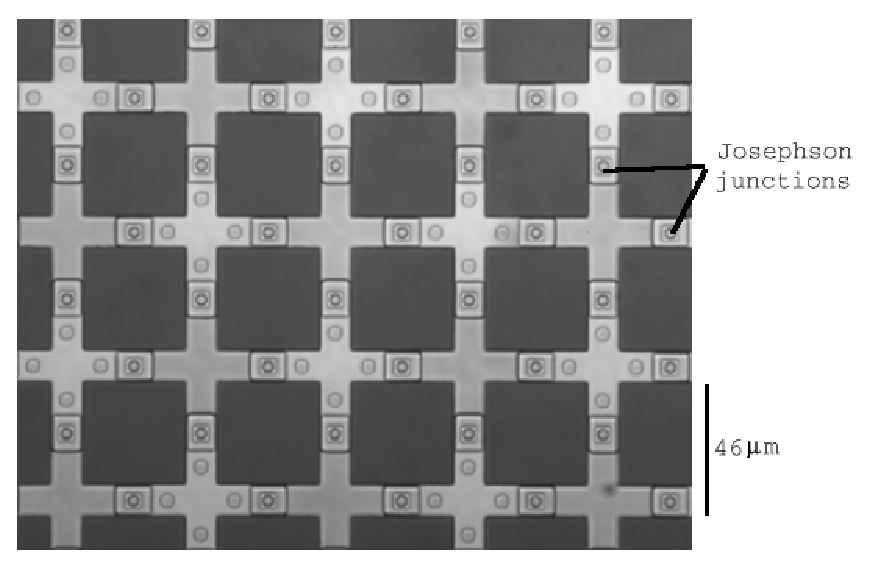
\includegraphics{figs/pme_exp/fig3_1.ps}
\caption[Optical micrograph of \jja\ samples used in the PME experiment.]
{Optical micrograph of several unit cells of the array showing
the crosses and locations of Josephson junctions. The unit cell size
is $46\,\micron$ and the wires are $10\,\micron$ across.
}
\label{fig:sample_sketch}
\end{figure}


\section{Experimental technique}
\label{sec:exp_method}

Kirtley \etal\,\cite{kirtley_jpcm_10_L97_1998}\ used a scanning SQUID
microscope (SSM), described in \InLineRef{kirtley_apl_66_1138_1995},
to image the BSCCO samples from Braunisch\etal 
\cite{braunisch_prl_68_1908_1992,braunisch_prb_48_4030_1993}\
and investigate the spatial distribution of paramagnetism in 
paramagnetic-superconducting BSCCO. This elegant experiment
provided inspiration for our work.

Our SSM has improvements over Kirtley's that make it ideally suited to
this type of experiment.\footnote{For a description of the 
experimental probe see
appendix \ref{chap:ssm_appendix}.} 
Our probe has a larger scanning 
range, as well as thermal isolation between the SQUID and the sample
(since they are not in direct contact).
 Kirtley \etal\ were unable to scan to the
edges of their sample, due to scanning stage restrictions. We are
able to scan over our entire sample, which proved to be crucial
to our analysis of the origin of PME. 
%Furthermore, there are artifacts
%in the Kirtley \etal\ data (\cf\ \InLineRef{kirtley_jpcm_10_L97_1998},\
%Fig.~1) due to the arrangement of the SQUID pickup coil which induces a
%false signal into the sample over the large area scanned. Because
%of our different SQUID arrangement we do not have this problem. 

The benefits of the SSM over more conventional magnetic measurement techniques 
are legion. The primary benefits arise from the fact that
the measured data are spatially resolved and the 
measurable field strengths are so low. 
Theories of PME
provide forms for the flux distribution
near the edges;%
\footnote{Theories of PME are discussed in the introductory material to
chapter \ref{chap:pme_theory}.} 
experimental verification
of these theories requires measurements of spatially-resolved magnetization. 
Other experimental techniques such as scanning Hall probe microscopy or
Magneto-Optical Indicator Films (MOIF) may be used to provide spatially
resolved information. However, both Hall probes and MOIF are not sensitive
to the magnetic field levels of interest in our arrays. 
One flux quantum per unit cell of the array has an average magnetic field
of $10^{-3}\,\mathrm{G}$ and we will typically measure 
signals on the order of
fractions of a single flux quantum. 

%
% fig 3.2
%
\begin{figure}[p]
\includegraphics{figs/pme_exp/fig3_2.eps}
\caption[Experimental arrangement of sample \jja\ and SQUID in the
probe.]{Experimental arrangement of sample \jja\ and SQUID at the cold
end of the scanning SQUID probe. The sample moves in $x$ and $y$
under the SQUID. Output signal from the SQUID is measured point by point
as the sample is scanned to generate an image of the magnetic induction
over the sample. The SQUID-sample separation is generally around 
$50\,\micron$. }
\label{fig:pme_experimental_setup}
\end{figure}

To run the experiment, \jja\ samples are placed on the end of the
cylindrical sample
stage cold finger, as shown in \FigRef{fig:pme_experimental_setup}. 
The cold finger is a $10\,\mathrm{mm}$ diameter sapphire 
rod around which a solenoid is wound. This solenoid provides the external
flux \Phiext\ to the sample. 

Prior to any measurement, the SQUID is adjusted
to insure that no flux is pinned in the body. This is accomplished by
first
thermal cycling the SQUID to remove trapped flux.  The
SQUID  is then scanned over a superconducting 
sample  (a technique developed in \InLineRef{mathai_phdthesis})
to observe if there is still
flux trapped in the SQUID, noting the sample 
response
as 
the SQUID is moved over the sample.
Eliminating the flux in the SQUID
minimizes the interaction between the SQUID and the sample and eliminates 
false signals that may result from
sample response to flux in the SQUID.

With the system cold,
we cannot easily know precisely how far apart the SQUID and the sample are.
To insure the SQUID does not collide with the sample, 
we rely on clues from the processed data. 
Sadly, many samples were lost due to the fact that 
the probe
provides no means to measure the separation \insitu. For a typical
scan discussed here, the SQUID -- sample separation is between
$40$ and $60\,\micron$. We infer this
because the lattice of the array is $46\,\micron$ and 
we can just begin to resolve array 
features in the data at this separation. For our
purposes we do not need to have unit cell resolution of the array,
nor will the exact measure of the SQUID -- sample separation affect the 
results. 

%
% somewhere we need to comment about the localization of the
% damage to the damaged regions... these pictures suck, so I'm cutting
% them out.
%
%It is important to not damage the array by allowing the 
%SQUID and sample to come into contact. \FigRef{fig:mag_array_scratches}\
%demonstrates the results of scratches accidentally introduced
%\insitu\ into the array,
%both in the magnetic image and also in the optical image, 
%\FigRef{fig:mag_array_scratches}(a) and (b) respectively, of the array. 
%Scratches destroy part of the array  affecting the magnetization
%properties of that part.

%
% figure was cut b/c the images were not clear. Instead I just say
% in the text what I tried to show with the images. 
%
% fig 3.3
%
%\begin{figure}
%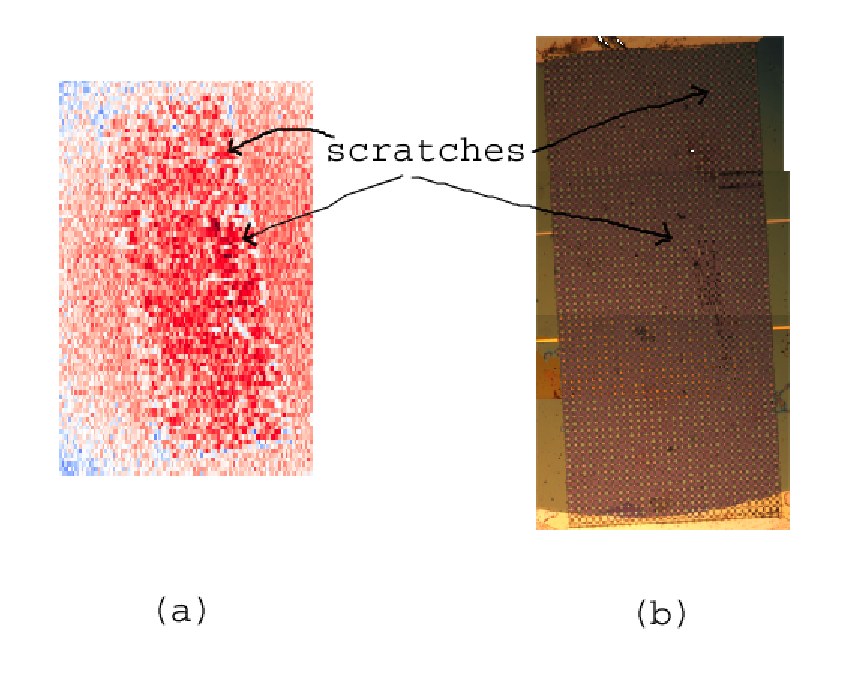
\includegraphics[width=5.7in]{figs/pme_exp/fig3_3.ps}
%\caption[Images of the $30\times 100$ junction array, 
%demonstrating \insitu\ scratches.]{(a) Magnetic image of the
%$30 \times 100$ junction array demonstrating accidental 
%\insitu\ scratches. (b) Optical micrograph of the same array
%showing the extent of the scratches.}
%\label{fig:mag_array_scratches}
%\end{figure}

After flux is removed from the SQUID, the sample is moved
so that the SQUID is far away (greater than
$10\,\mathrm{mm}$, in $x$ and $y$, not $z$) 
in order to 
avoid any possible interference between the SQUID and the sample during 
field cooling. \FigRef{fig:ZFC_with_close_SQUID} shows the effect of zero
field cooling the sample with the SQUID positioned over the middle of the 
$30 \times 100$ \jja. Flux became trapped in the sample in a similar pattern
to the wire arrangement on the surface of the SQUID tip, \cf\ 
\FigRef{fig:SQUID_optical_close}. 
It was found that turning off the SQUID, field cooling and
then reactivating the SQUID tended to trap flux in the sample when the 
feedback circuit was adjusted. 
To avoid this problem the SQUID was moved far away 
from the sample
until it had no noticeable effect when the sample was
zero field cooled.


% we want to arrange so that all color figures are on odd pages,
% or back to back, odd then even

\newcommand{\figthreefour}{
% in principle, this command will insert figure 3.4 right here
%
% fig 3.4 - color figure
%
\begin{figure}[p]
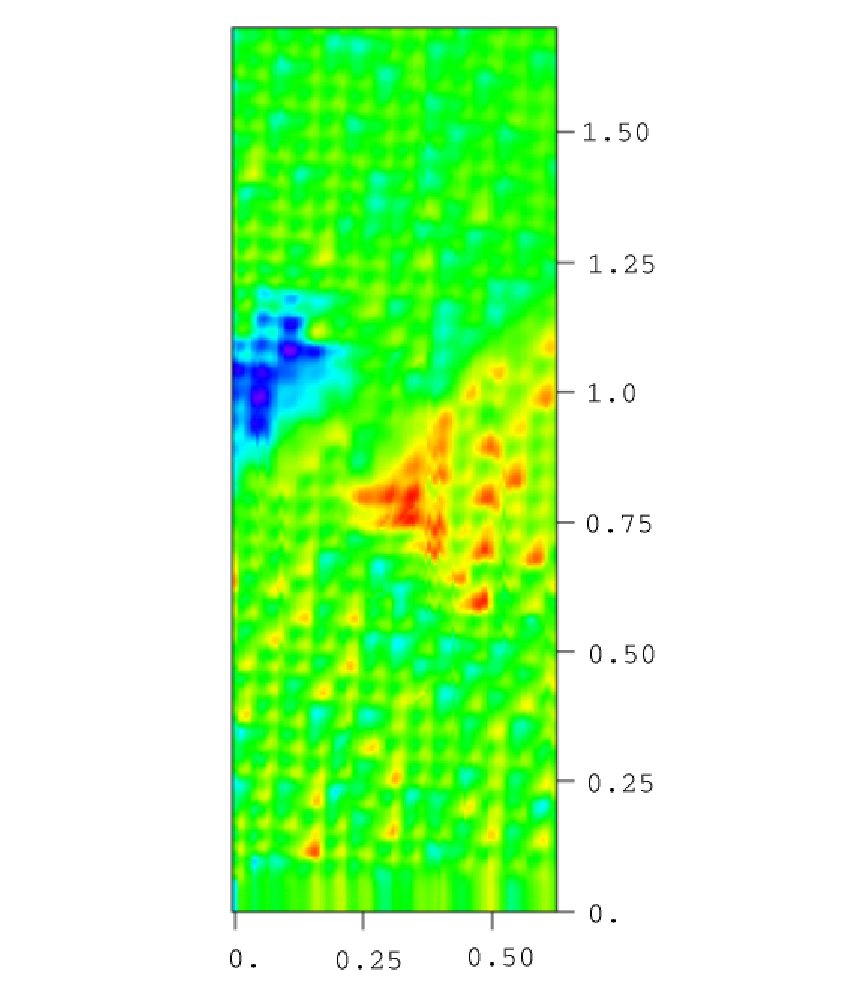
\includegraphics{figs/pme_exp/fig3_4r2.ps}
\caption[Zero-field cooled, with SQUID on top, magnetic image of sample.]{
Zero field cooled magnetic image of $30 \times 100$ \jja, with the 
SQUID positioned in the
middle of the sample during cooling. 
The color scale represents a range from purple (low) to red (high) of
$8 \Phinot$ per unit cell of the array and the $x$ and $y$ units are 
shown in millimeters. 
The flux trapped in the 
array is due to the currents flowing in the SQUID and feedback 
coil wires on the SQUID tip.
The smeared out data near $x=0$ is a mechanical artifact.} 
\label{fig:ZFC_with_close_SQUID}
\end{figure}
}

\ifthenelse{\isodd{\value{page}}}{\figthreefour}{\afterpage{\figthreefour}}

In practice, I begin taking measurements by
heating the sample above $T_c = 9.2\,\kelvin$
to $13\,\kelvin$. We then apply an external flux to the sample and remove
the heat source. The sample cools in field to $4.2\,\kelvin$ and the
measurement begins. 

Each measurement of a magnetization image 
consists of four scanning passes of the SQUID over the sample
in different situations.
Each scanning pass produces an image of the flux threading the SQUID at a 
particular point in space above the sample. 
\FigRef{fig:pme_scanning_passes_a} through 
\FigRef{fig:pme_scanning_passes_d}\ shows 
representative images of the four scanning passes made over the sample
to produce the magnetization image. 
We wish to compute the magnetization of the sample. In MKS units,
\begin{equation}
\vec{M}=\left( \vec{H}-{1 \over \mu_0} \vec{B} \right)\mathrm{.}
\label{eqn:magnetization_defn}
\end{equation}
The magnetization vector $\vec{M}$
can be related to a flux through an area
\begin{equation}
\Phimag = \mu_0 \int_A \vec{M}\cdot \dif \vec{a}
\end{equation}
just as $\vec{B}$ and $\vec{H}$ are associated with a flux through a 
particular area
\begin{eqnarray}
\Phitot & = & \int_A \vec{B}\cdot \dif \vec{a} \\
\Phiext & = & \mu_0 \int_A \vec{H}\cdot \dif \vec{a} \mathrm{.}
\end{eqnarray}
so that \EqnRef{eqn:magnetization_defn} can be expressed in terms of 
flux
\begin{equation}
\Phimag = \Phitot - \Phiext \mathrm{.}
\label{eqn:magnetization_flux_defn}
\end{equation}


%
% fig 3.5
%
%\begin{figure}[p]
%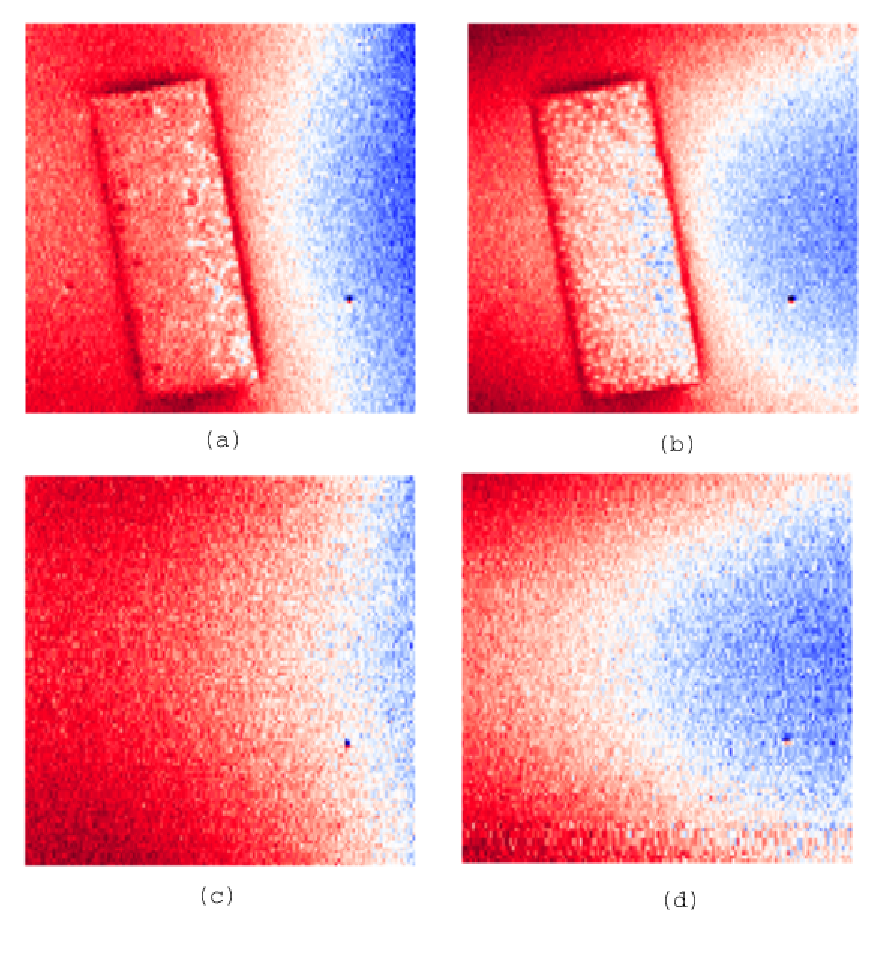
\includegraphics[width=5.7in]{figs/pme_exp/fig3_5r2.ps}
%\caption[Representative magnetic images from the four scanning passes
%required to determine the field cooled array magnetization.]{
%Representative images from the four scanning passes made in
%order to determine the magnetization of the field cooled sample.
%In each image the colors range from blue (low) to red (high) for 
%a total flux difference of $0.17\,\Phinot$ per unit cell of the
%array. Each image is $5\times 5\,\mathrm{mm}$ square. 
%(a) Magnetic image of sample after field cooling in $\phiext = 4.8$,
%$T=4.2\,\kelvin$.
%(b) Magnetic image of zero field cooled sample, $T=4.2\,\kelvin$. 
%(c) Magnetic image of $\phiext = 4.8$, $T=13\,\kelvin$. (d) Magnetic
%image of zero field, $T=13\,\kelvin$. }
%\label{fig:pme_scanning_passes}
%\end{figure}


\begin{figure}[p]
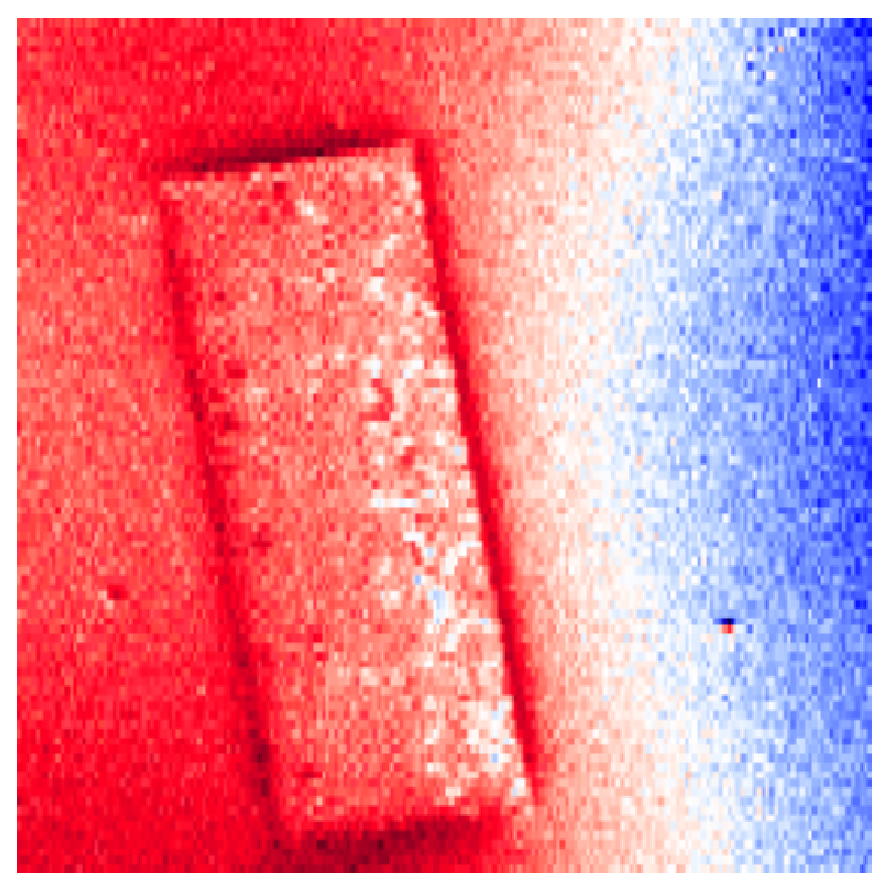
\includegraphics[width=5.7in]{figs/pme_exp/fig3_5_a_lg.ps}
\caption[Magnetic image of sample after field cooling in $\phiext = 4.8$,
$T=4.2\,\kelvin$.]{
Magnetic image of sample after field cooling in $\phiext = 4.8$,
$T=4.2\,\kelvin$.
The colors range from blue (low) to red (high) for 
a total flux difference of $0.17\,\Phinot$ per unit cell of the
array. Each image is $5\times 5\,\mathrm{mm}$ square.}
\label{fig:pme_scanning_passes_a}
\end{figure}

\begin{figure}[p]
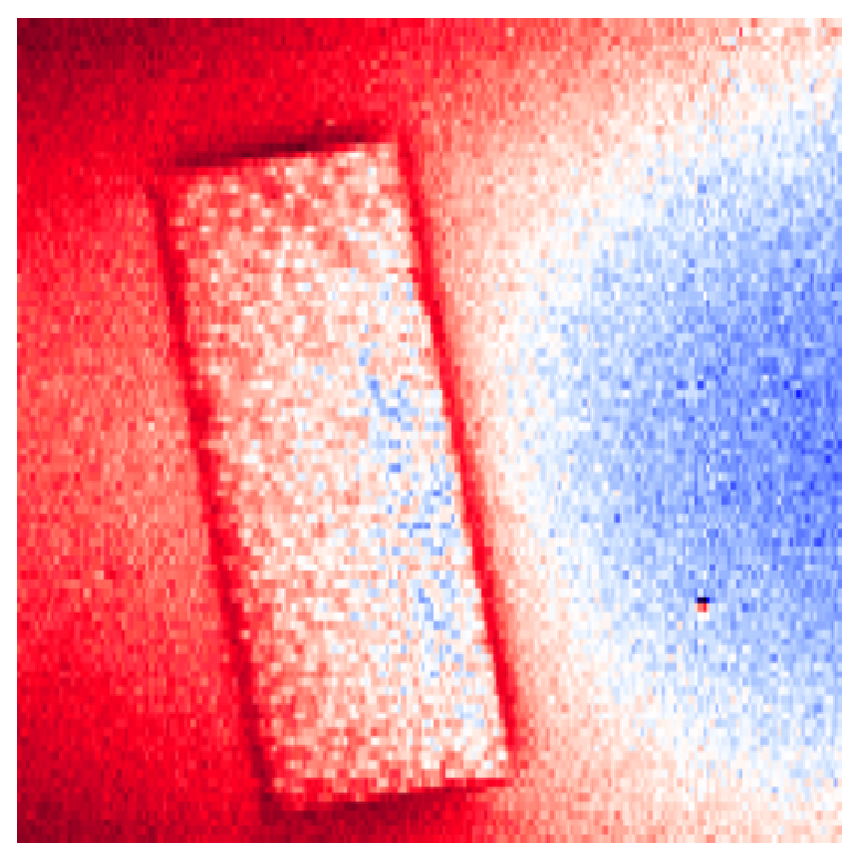
\includegraphics[width=5.7in]{figs/pme_exp/fig3_5_b_lg.ps}
\caption[Magnetic image of zero field cooled sample, $T=4.2\,\kelvin$.]{
Magnetic image of zero field cooled sample, $T=4.2\,\kelvin$.
The colors range from blue (low) to red (high) for 
a total flux difference of $0.17\,\Phinot$ per unit cell of the
array. Each image is $5\times 5\,\mathrm{mm}$ square.}
\label{fig:pme_scanning_passes_b}
\end{figure}

\begin{figure}[p]
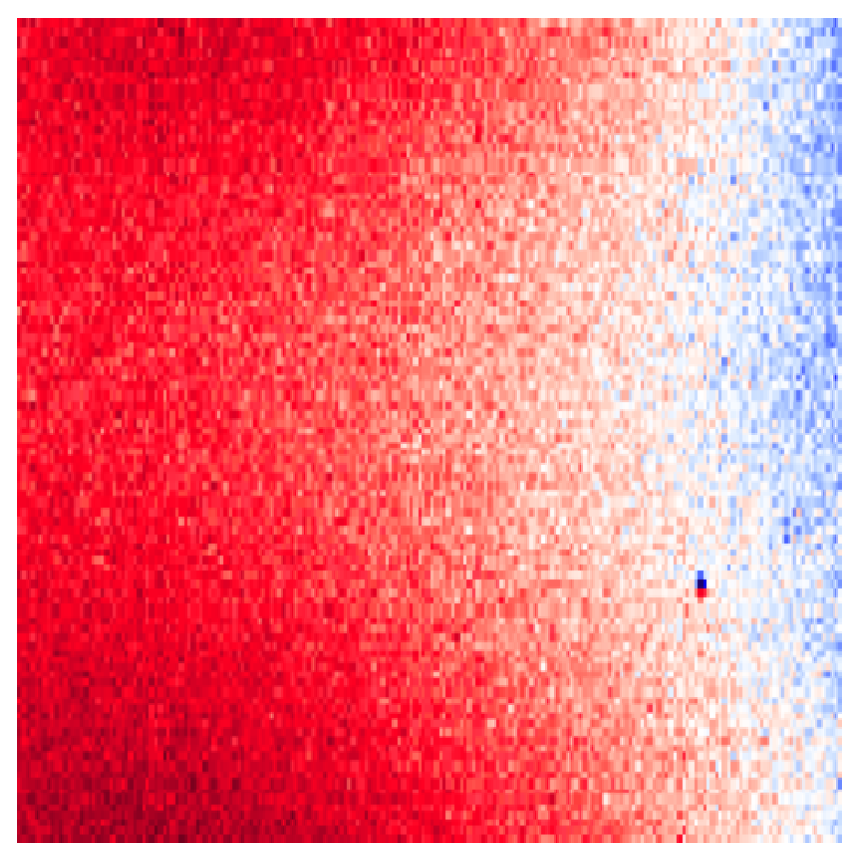
\includegraphics[width=5.7in]{figs/pme_exp/fig3_5_c_lg.ps}
\caption[Magnetic image of $\phiext = 4.8$, $T=13\,\kelvin$.]{
Magnetic image of $\phiext = 4.8$, $T=13\,\kelvin$.
The colors range from blue (low) to red (high) for 
a total flux difference of $0.17\,\Phinot$ per unit cell of the
array. Each image is $5\times 5\,\mathrm{mm}$ square.}
\label{fig:pme_scanning_passes_c}
\end{figure}

\begin{figure}[p]
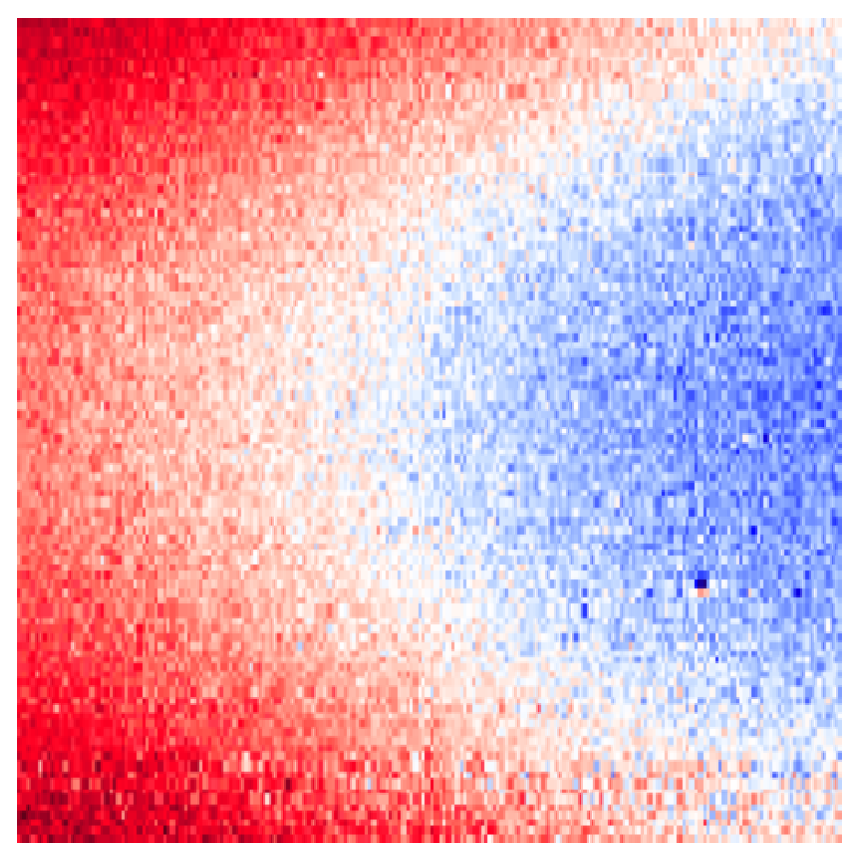
\includegraphics[width=5.7in]{figs/pme_exp/fig3_5_d_lg.ps}
\caption[Magnetic
image of zero field, $T=13\,\kelvin$.]{
Magnetic
image of zero field, $T=13\,\kelvin$. 
The colors range from blue (low) to red (high) for 
a total flux difference of $0.17\,\Phinot$ per unit cell of the
array. Each image is $5\times 5\,\mathrm{mm}$ square.}
\label{fig:pme_scanning_passes_d}
\end{figure}


%
% fig3.6
%
%\begin{figure}[p]
%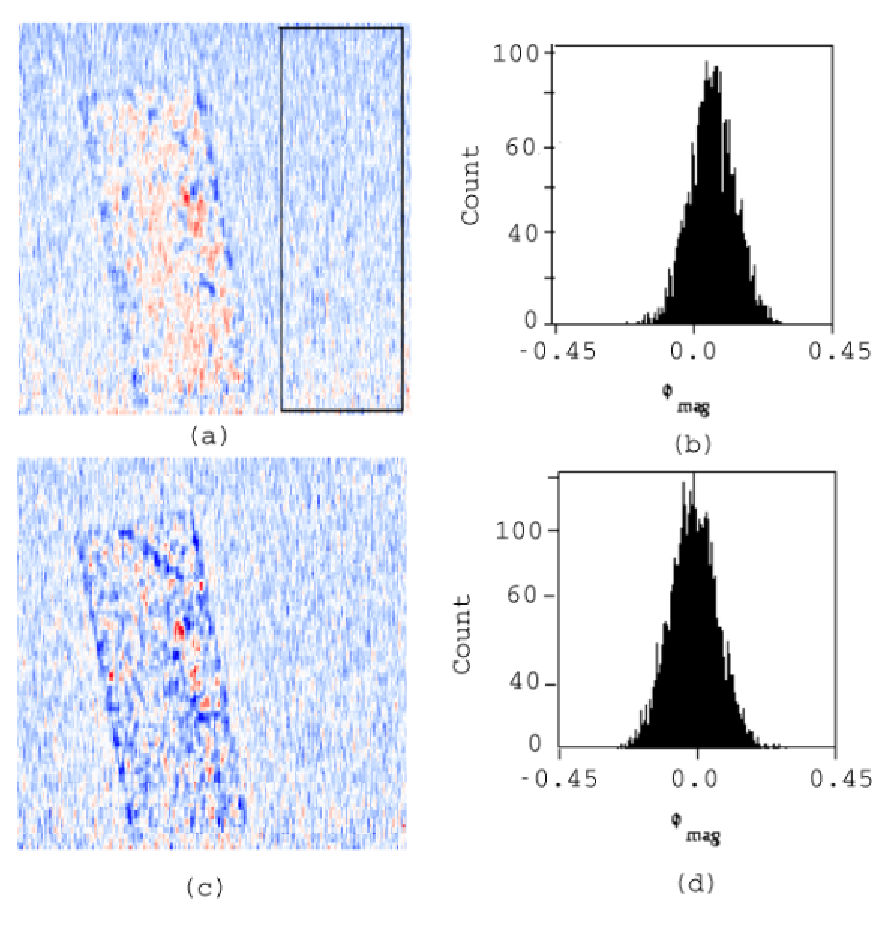
\includegraphics[width=5.7in]{figs/pme_exp/fig3_6.ps}
%\caption[Magnetization images of a field cooled $30\times 100 $ array.]{
%(a) Magnetization of $30\times 100$ junction array after field
%cooling in $\phiext = 4.8$. (b) Histogram of the magnetization data shown
%in the magnetization image (a). (c) Magnetization of array after field
%cooling in $\phiext = 1.2$. (d) Histogram of the magnetization data shown in 
%magnetization image (c). For both of the magnetization images the color 
%ranges from red, $\phimag = 0.45$ (paramagnetic) 
%to blue, $\phimag = -0.45$ (diamagnetic). The long side of the array
%is $4.6\,\mathrm{mm}$ long. 
%}
%\label{fig:paramag_image}
%\end{figure}

\begin{figure}[p]
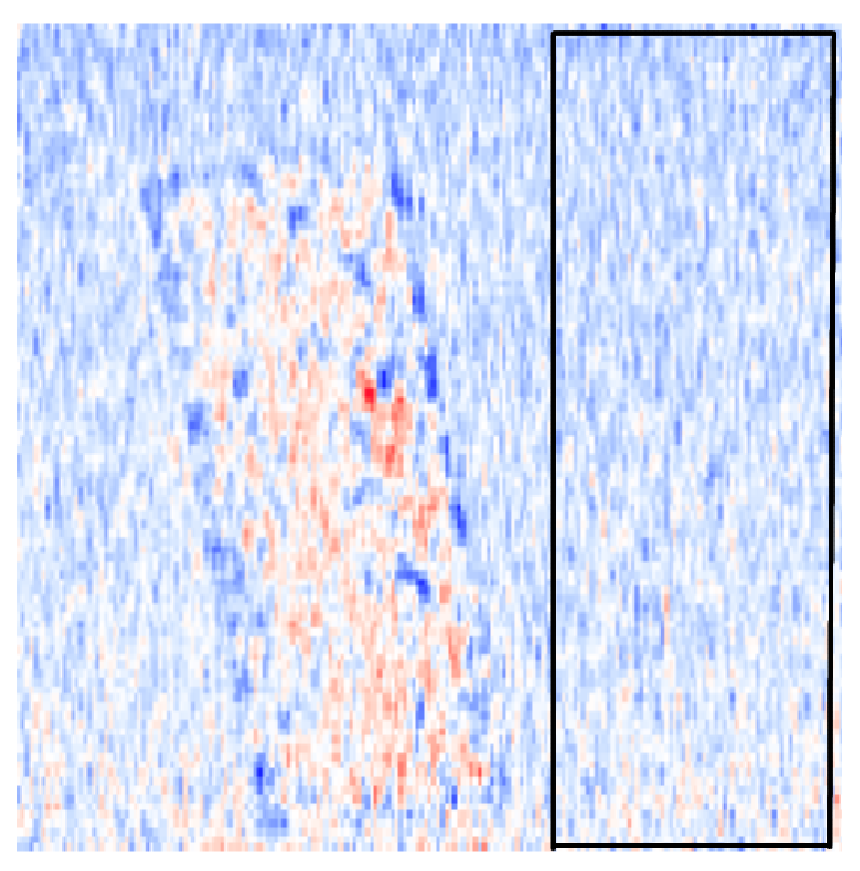
\includegraphics[width=5.7in]{figs/pme_exp/fig3_6_a_lg.ps}
\caption[Magnetization of $30\times 100$ junction array after field
cooling in $\phiext = 4.8$.]
{Magnetization of $30\times 100$ junction array after field
cooling in $\phiext = 4.8$. The color 
ranges from red, $\phimag = 0.45$ (paramagnetic) 
to blue, $\phimag = -0.45$ (diamagnetic). The long side of the array
is $4.6\,\mathrm{mm}$ long. }
\label{fig:paramag_image_a}
\end{figure}

\begin{figure}[p]
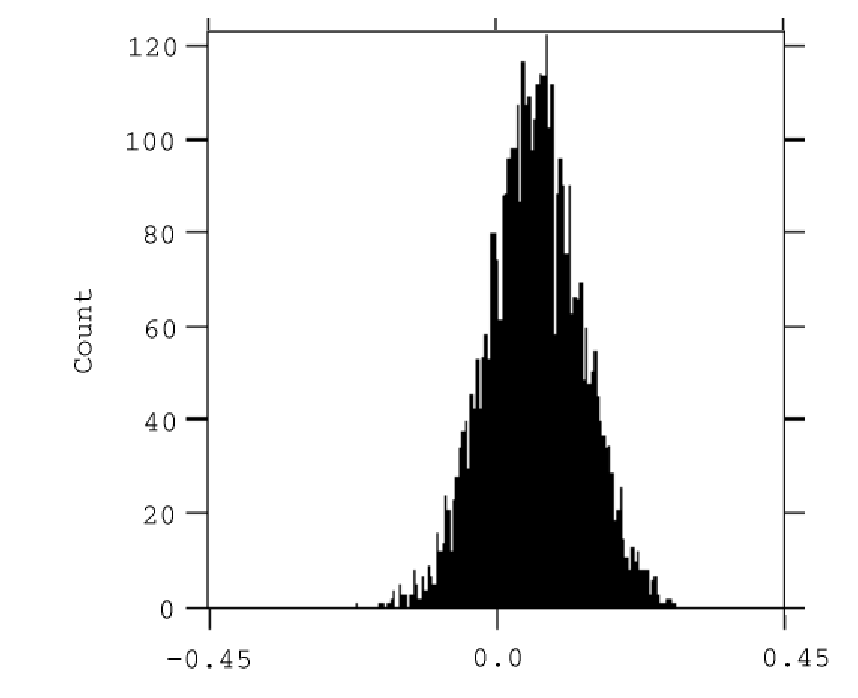
\includegraphics[width=5.7in]{figs/pme_exp/fig3_6_b_lg.ps}
\caption{Histogram of the magnetization data shown
in the magnetization image, \FigRef{fig:paramag_image_a}.}
\label{fig:paramag_image_b}
\end{figure}

\begin{figure}[p]
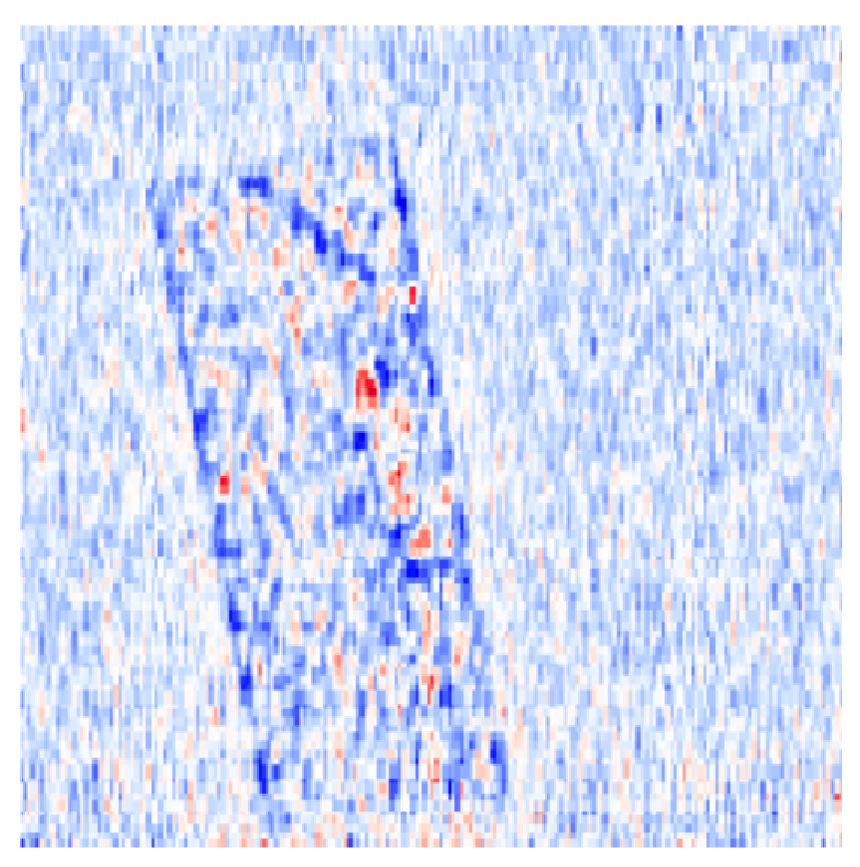
\includegraphics[width=5.7in]{figs/pme_exp/fig3_6_c_lg.ps}
\caption[Magnetization of $30\times 100$ junction array after field
cooling in $\phiext = 1.2$.]{Magnetization of $30\times 100$ 
junction array after field
cooling in $\phiext = 1.2$. The color 
ranges from red, $\phimag = 0.45$ (paramagnetic) 
to blue, $\phimag = -0.45$ (diamagnetic). The long side of the array
is $4.6\,\mathrm{mm}$ long. }
\label{fig:paramag_image_c}
\end{figure}

\begin{figure}[p]
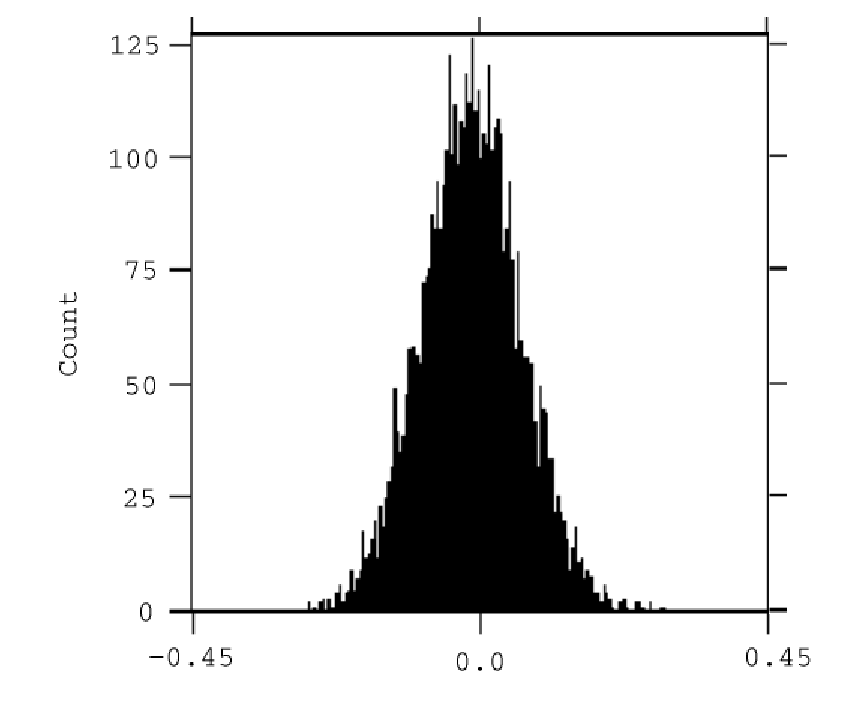
\includegraphics[width=5.7in]{figs/pme_exp/fig3_6_d_lg.ps}
\caption{Histogram of the magnetization data shown
in the magnetization image, \FigRef{fig:paramag_image_c}.}
\label{fig:paramag_image_d}
\end{figure}

If there were no systematic position-dependent errors,
we would need only measure the field-cooled image to 
get \Phitot\ and the image of the field at $13\,\kelvin$ to get \Phiext.
\index{heating}\index{friction}
However,
friction in the plastic scanning mechanism generates heat that  
does not dissipate
quickly into the \lhe\ bath and
warms both the SQUID and the sample by slightly less than $1\,\kelvin$. 
This change in the sample temperature
does not matter. The sample never
warms to the point where thermal activation can overcome the energy
barriers due to the array's Hamiltonian, \EqnRef{eqn:array_hamiltonian}. 
Conversely, the heating of the SQUID is important.
 
\FigRef{fig:squid_vs_temperature} shows how the SQUID output changes 
during a $1\,\kelvin$ temperature change. This change is comparable to the
signal level shown 
in \FigRef{fig:pme_scanning_passes_a}\ through
\FigRef{fig:pme_scanning_passes_d}, so the heating of the SQUID must be
considered in order to validate the results. 
This heating effect depends upon the
sample position because the friction changes during different parts of a
scan. Consequently, each image of the sample will
measure two things, the real flux threading the SQUID \Phitot\
and a false
``flux'' distribution $\Phi_\mathrm{Friction\,@\,4.2\,K}$ 
due to the position-dependent heating.
The false flux distribution will be
different at different temperatures since
the 
sample's 
temperature causes a noticeable heat load
on the SQUID.  

It is further possible that after eliminating the flux from the SQUID
that there might be some background flux impinging upon the sample. 
This is clear in the zero field-cooled image, 
\FigRef{fig:pme_scanning_passes_b}, in which some array response
is evident despite the lack of applied field. This false flux
signal
will be a time-independent $\Phi_\mathrm{background}$ in all the images in
\FigRef{fig:pme_scanning_passes_a}\ through
\FigRef{fig:pme_scanning_passes_d} and will just subtract out. 

The total field-cooled flux in \FigRef{fig:pme_scanning_passes_a}\
thus
contains three sources, the real \Phitot, a false flux reading
in the SQUID due to friction,
and the background flux, so that
%
\begin{equation}
\Phi_\mathrm{FC} = \Phitot + \Phi_\mathrm{Friction\,@\,4.2\,K}
 + \Phi_\mathrm{background}.
\label{eqn:phi_fc}
\end{equation}
%
The total zero field-cooled flux in \FigRef{fig:pme_scanning_passes_b}\ 
also contains a false flux signal due to friction and the background flux
%
\begin{equation}
\Phi_\mathrm{ZFC} =  \Phi_\mathrm{Friction\,@\,4.2\,K}
 + \Phi_\mathrm{background}.
\end{equation}
%
The total measured high-temperature flux in 
\FigRef{fig:pme_scanning_passes_c}\ also contains a false flux due to 
friction. The magnitude 
is different because the SQUID sees a different heat load
due to the higher temperature of the sample,
%
\begin{equation}
\Phi_\mathrm{HT} = \Phiext  + \Phi_\mathrm{Friction\,@\,13\,K}
 + \Phi_\mathrm{background}.
\end{equation}
%
The measured zero-field, high-temperature flux in 
\FigRef{fig:pme_scanning_passes_d}\ is
%
\begin{equation}
\Phi_\mathrm{ZHT} =  \Phi_\mathrm{Friction\,@\,13\,K}
 + \Phi_\mathrm{background}.
\label{eqn:phi_zht}
\end{equation}
%
Eqns.~(\ref{eqn:phi_fc}) - (\ref{eqn:phi_zht}) 
combine to give the total sample magnetization
\begin{equation}
\Phimag = \Phitot - \Phiext = (\Phi_\mathrm{FC} - \Phi_\mathrm{ZFC})-
                              (\Phi_\mathrm{HT} - \Phi_\mathrm{ZHT}).
\label{eqn:mag_correction}
\end{equation}

\FigRef{fig:paramag_image_a}\
shows the magnetization image resulting from the four passes
given in \FigRef{fig:pme_scanning_passes_a}\ through
\FigRef{fig:pme_scanning_passes_d} after applying 
\EqnRef{eqn:mag_correction} to the data. The red colors in the image
represent $M>0$, a paramagnetic magnetization and the blue colors 
represent $M<0$, a diamagnetic magnetization. Qualitatively 
the interior of the array
is more \emph{red} than blue, hence it is paramagnetic. 

For each scan, data are collected every $5\,\micron$ in the $x$ direction
and every $50\,\micron$ in the $y$ direction. The discrepancy between 
data collection in $x$ and $y$ direction results from the scanning
mechanism. The scan lines are in the $x$ direction while the raster
lines are in the $y$ direction. Each image in 
\FigRef{fig:pme_scanning_passes_a}\
through \FigRef{fig:pme_scanning_passes_d}
took approximately 45 minutes to complete. 
Each magnetization measurement must be completed before
the \lhe\ boils out of the Dewar, which has a hold time of 11 to 12 hours.
In order to make several magnetization measurements to check consistency
it would be prohibitive to increase the amount of time required for each
scan. 

\section{Experimental results}

\subsection[$30 \times 100$ junction array]
{$\mathbf{30 \times 100}$ junction array}

We first looked at a $30 \times 100$ \jja\ performing field cooled 
measurements of the type
described above in 
Section \ref{sec:exp_method}. We determined that the array could be 
either paramagnetic or diamagnetic depending upon the cooling field. 
\FigRef{fig:paramag_image_a}\ through
\FigRef{fig:paramag_image_d}\ demonstrates the results of field cooling 
for the array for two external fields, $\phiext = 1.2$ and $\phiext = 4.8$. 
The colors in \FigRef{fig:paramag_image_a}\ and
\FigRef{fig:paramag_image_c}\ represent the magnetization
in the image at each point. 
The colors range from 
red, $\phimag = 0.45$ (paramagnetic data)
to blue, $\phimag = -0.45$ (diamagnetic data).%
\footnote{Recall the definitions made in \EqnRef{eqn:dimensionless_subs}
that $\phi = \Phi/\Phi_0$.}
By looking at the images in \FigRef{fig:paramag_image_a}\
we can qualitatively see that the
array is overall paramagnetic, since it is more red,
although the magnetization
is clearly quite complicated. In \FigRef{fig:paramag_image_c}
the array is overall diamagnetic, since it is more blue. 

There is an additional important feature to note which appears in all of the
magnetization images collected, regardless of the overall array magnetization.
The array always has a diamagnetic screening current (shown in the images
as a blue loop) around the outside
edge, \cf\ \FigRef{fig:paramag_image_a}\  and \FigRef{fig:paramag_image_c}. 

In order to make a quantitative analysis,
we looked at histograms of the individual magnetization images.
For this $30 \times 100$ array, we looked only at the bottom one third
of the array because scratches were accidentally introduced into the 
array \textit{in situ} which produce anomalous results. 
The extent of the
anomalous magnetization due to the scratches matches up well with the 
actual extent of the scratches as observed under the optical microscope.
Because of the close correlation between the location of the scratches
in the magnetic and optical images, it was concluded that the scratches
did not affect the magnetization results very far from the area of the
scratches. 

Histograms for \FigRef{fig:paramag_image_a}\ and \FigRef{fig:paramag_image_c} 
are shown in 
\FigRef{fig:paramag_image_b}\ and \FigRef{fig:paramag_image_d} 
respectively. These two histograms
are representative of the histograms generated for all the data on 
this array. For \FigRef{fig:paramag_image_a}, field cooled
at $\phiext = 4.8$, the mean of \FigRef{fig:paramag_image_b} is 
$\langle\phimag\rangle = 0.068$ with a standard deviation of 
$\sigma = 0.15$,
clearly
greater than zero, so the array is overall paramagnetic. Similarly for
\FigRef{fig:paramag_image_c}, field cooled at $\phiext = 1.2$, 
the mean of \FigRef{fig:paramag_image_d} is 
$\langle\phimag\rangle= -0.016$ with a standard deviation of 
$\sigma = 0.16$,
clearly less than
zero, so the array is overall diamagnetic. 
Interestingly, the histogram data for all of the cooling fields have similar
widths, $\sigma \approx 0.15$. 

%
% fig3.7 - background histograms
%
%\begin{figure}[p]
%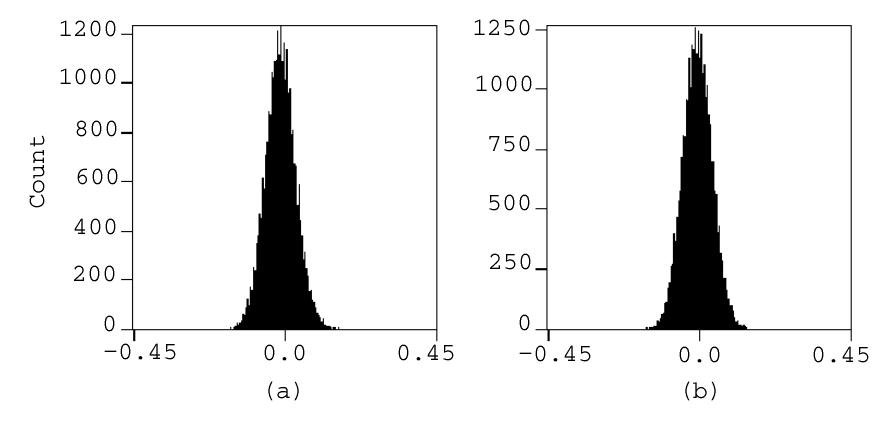
\includegraphics[width=5.7in]{figs/pme_exp/fig3_7.ps}
%\caption[Histograms of the magnetization background.]{Histograms of the 
%magnetization background for the images in \FigRef{fig:paramag_image_a}
%and \FigRef{fig:paramag_image_c}. 
%(a) Histogram of background magnetization for $\phiext = 4.8$. (b)
%Histogram of background magnetization for $\phiext = 1.2$.}
%\label{fig:hist_background}
%\end{figure}

\begin{figure}[p]
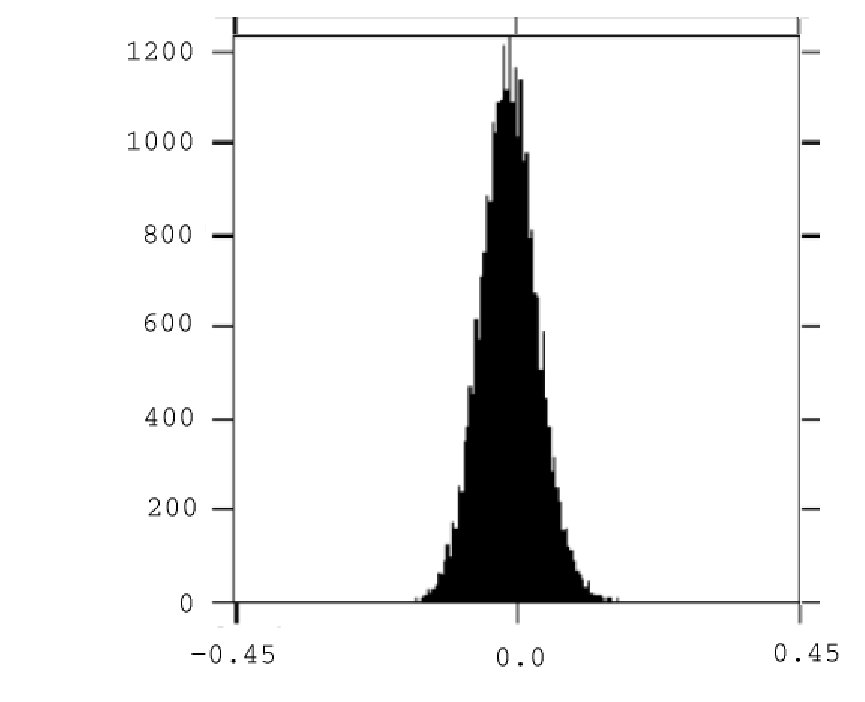
\includegraphics[width=5.7in]{figs/pme_exp/fig3_7_a_lg.ps}
\caption{Histogram of background magnetization for $\phiext = 4.8$, from
\FigRef{fig:paramag_image_a}.}
\label{fig:hist_background_a}
\end{figure}

\begin{figure}[p]
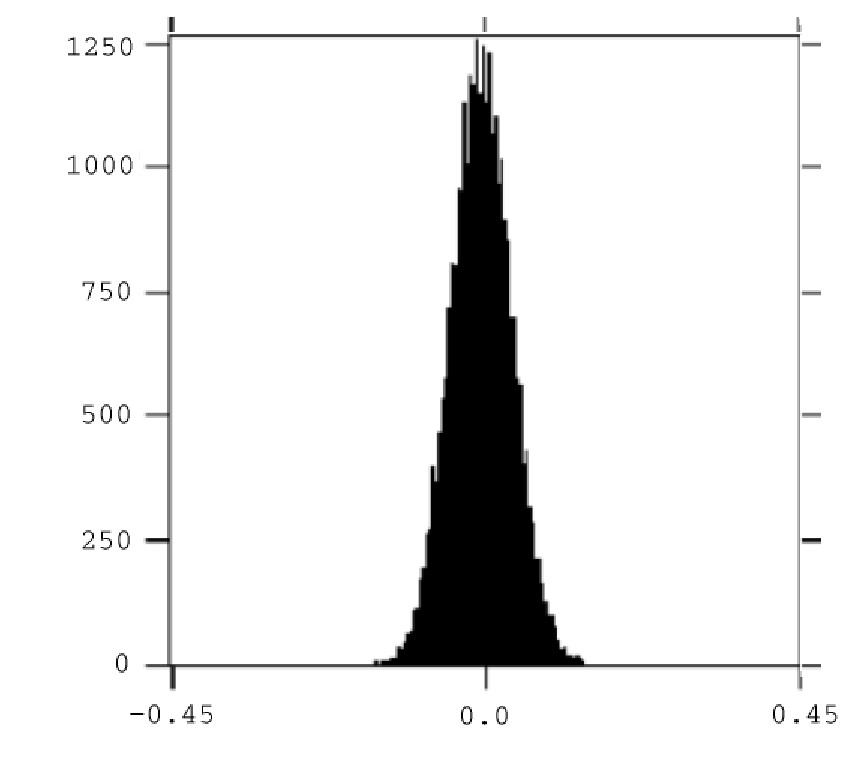
\includegraphics[width=5.7in]{figs/pme_exp/fig3_7_b_lg.ps}
\caption{Histogram of background magnetization for $\phiext = 1.2$, from
\FigRef{fig:paramag_image_c}.}
\label{fig:hist_background_b}
\end{figure}



%
% back ground discussion
%
In each magnetization image, \FigRef{fig:paramag_image_b} and 
\FigRef{fig:paramag_image_d}, a region, 
indicated by a box, was analyzed to 
determine the magnetization of the background. We carried out this
analysis by generating histograms for the background, similar to the
histograms for the array. 
These background histograms are shown 
in \FigRef{fig:hist_background_a} and \FigRef{fig:hist_background_b} 
respectively. 
It is readily apparent from the comparison that the width of the 
background histograms is approximately one-half that of the 
array histograms, and that the mean of the background histograms
is $\langle\phimag\rangle=0.00$ with a standard deviation of
$\sigma = 0.08$, in contrast to the array histograms which
have clear non-zero mean values and $\sigma = 0.15$. 

We have repeated the same types of measurements on this array for 
many different values of the cooling field. These results are 
summarized in \FigRef{fig:sm_array_mag_plot}, which shows the 
measured mean magnetization of the array plotted versus the cooling
field used. Note that the array magnetization is multivalued for some
values of the cooling field. More importantly, although the array may
be diamagnetic for small values of \phiext, it is increasingly
paramagnetic with increasing values of the external field. 
Note that the magnetization curves, as discussed in chapter~\ref{chap:jjarray},
p.~\pageref{jjarray:single_loop_mag}, are very steep for a single loop,
so small variations in \phiext\ may lead to large variations in \phimag\
which could lead to our multivalued solutions. Additionally, we can
see from \EqnRef{eqn:steadystatesolution}\ that a single loop has 
many different solutions for a given \phiext\ so it is not 
unreasonable to think that the array might have multivalued
solutions for a given \phiext\ as well. In fact because the
array is more complicated than a single loop, one might 
expect it to likely be frustrated during field
cooling and to end up in different states for the
same cooling field. 

The range of flux in 
\FigRef{fig:paramag_image_d} (zero field, $T=13\,\kelvin$)
is $0.17\,\Phinot$ per unit cell of the 
array, so we can be confident that the actual gradient of 
the background field is at least this small, meaning that the
array sees flux uniform to $\phiext \pm 0.17$. 
This variation in \phiext\ corresponds to a potential variation
in magnetization of $\pm 0.05$ by comparing with 
\EqnRef{eqn:steadystatesolution}.

Because of the large number of data points that went into computing the 
averages for \FigRef{fig:paramag_image_b} we find
a mean paramagnetic response of $\phimag = 0.063\pm 0.005$.
and for \FigRef{fig:paramag_image_d} we find a mean diamagnetic
response of $\phimag = -0.016 \pm 0.005$. This is a larger
variation than the control we have with the current source to the
solenoid, a Keithley 224 programmable current source
\cite{keithley_instr}.

\begin{figure}[p]
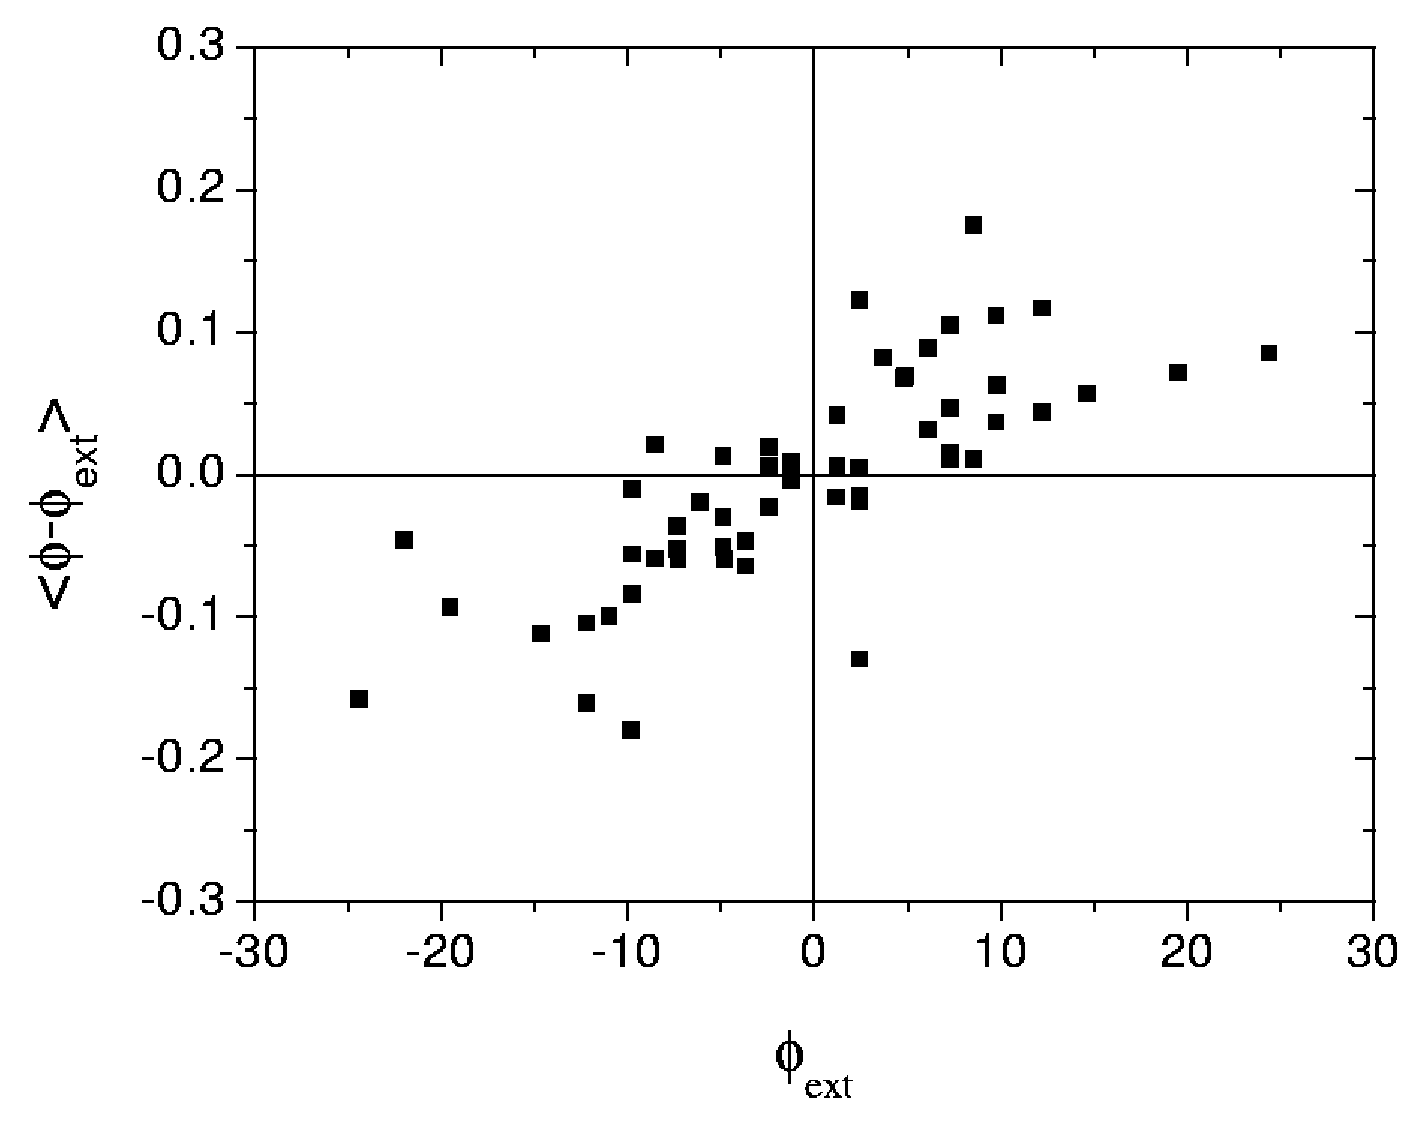
\includegraphics[width=5.7in,keepaspectratio=true]{figs/pme_exp/fig3_8.eps}
\caption[Measured mean magnetization for $30 \times 100$ junction
array plotted versus cooling field.]{Measured mean magnetization
for $30 \times 100$ junction array plotted versus cooling field.
The error in each data point is less than the size of the symbol.}
\label{fig:sm_array_mag_plot}
\end{figure}

\subsection[$100 \times 150$ junction array]
{$\mathbf{100 \times 150}$ junction array}

In addition to the $30 \times 100$ junction array, we were interested
to see 
what effect the geometry of the sample might have upon the measured
magnetization because some theories predict that 
the size of the
sample is important to the paramagnetic response
\cite{geim_nature_396_144_1998,koshelev_prb_53_13559_1995}. 
For this purpose,
we chose to 
look at an array of 
$100 \times 150$ \jjsnoun. This array was otherwise exactly the same as the 
previous $30 \times 100$ junction array and the 
magnetization measurements were
carried out in the same way. 

An 
image showing a paramagnetic state of the larger array is shown
in \FigRef{fig:lg_paramag_image_a} with the corresponding
histogram shown in \FigRef{fig:lg_paramag_image_b}. 
In this data set, for an applied field of $\phiext = -11.0$
the response was paramagnetic, $\phimag = -0.099 \pm 0.005$.
There were
no \insitu\ scratches accidentally introduced into this array, 
however, there was some noise in the SQUID output, present as the
straight horizontal line, in the top of the image,
so we 
were able to analyze the magnetization histogram for the entire array,
except for the noisy region.  

%\begin{figure}[p]
%\includegraphics[width=5.7in]{figs/pme_exp/fig3_9.eps}
%\caption[Paramagnetic image and histogram for $100\times 150$
%junction array.]{Representative paramagnetic image (a) and histogram (b)
%for the $100\times 150$ junction array. The array was field cooled
%in a field of $\phiext = -11.0$. The color scale ranges from blue
%($-0.45\,\Phinot$) to red ($0.20\,\Phinot$) and the short side of
%the array is $4.6\,\mm$ long. 
% }
%\label{fig:lg_paramag_image}
%\end{figure}

\begin{figure}[p]
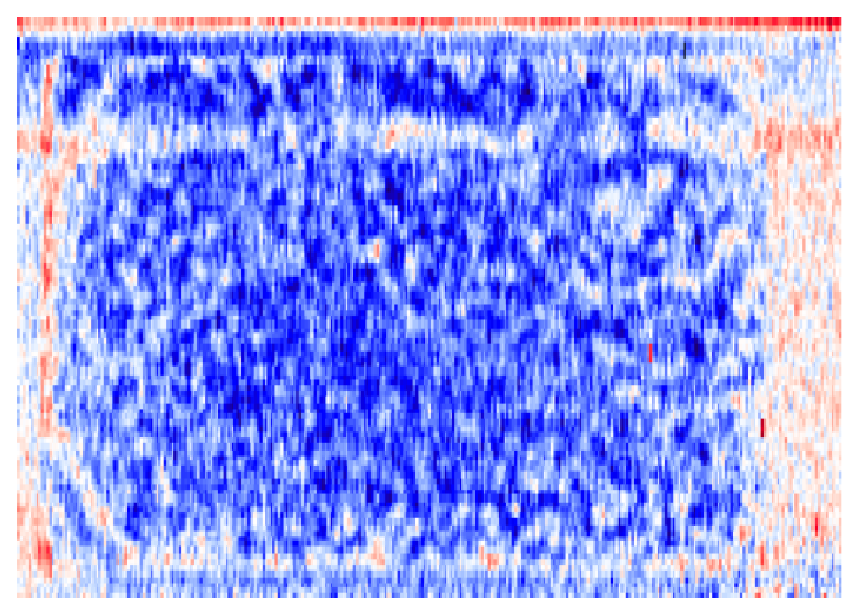
\includegraphics[width=5.7in]{figs/pme_exp/fig3_9_a_lg.ps}
\caption[Representative paramagnetic image
for the $100\times 150$ junction array.]{Representative paramagnetic image
for the $100\times 150$ junction array. The array was field cooled
in a field of $\phiext = -11.0$. The color scale ranges from blue
($-0.45\,\Phinot$) to red ($0.20\,\Phinot$) and the short side of
the array is $4.6\,\mm$ long. }
\label{fig:lg_paramag_image_a}
\end{figure}

\begin{figure}[p]
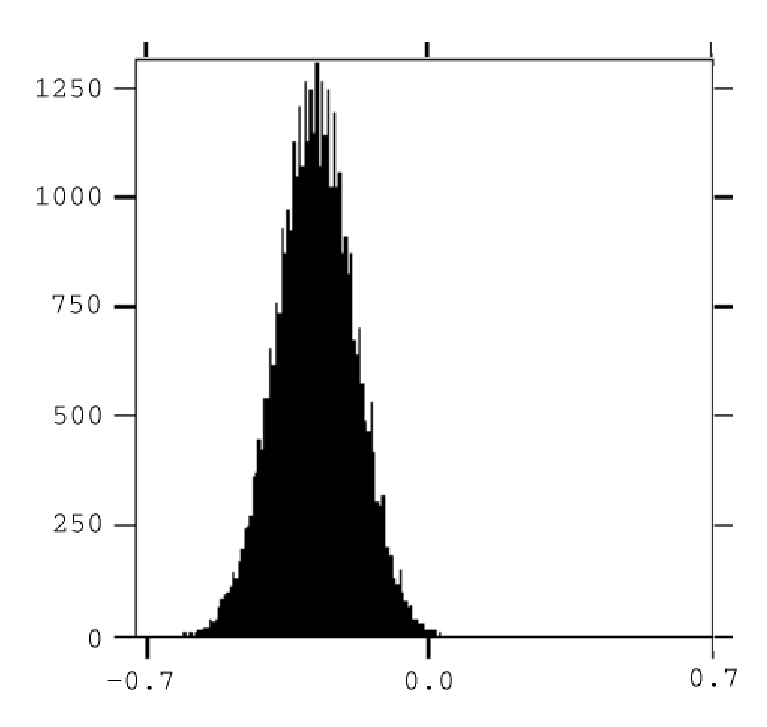
\includegraphics[width=5.7in]{figs/pme_exp/fig3_9_b_lg.ps}
\caption[Paramagnetic histogram shown in \FigRef{fig:lg_paramag_image_a}.]
{Paramagnetic histogram shown in \FigRef{fig:lg_paramag_image_a}.
The array was field cooled
in a field of $\phiext = -11.0$. The color scale ranges from blue
($-0.45\,\Phinot$) to red ($0.20\,\Phinot$) and the short side of
the array is $4.6\,\mm$ long. }
\label{fig:lg_paramag_image_b}
\end{figure}



The results from this measurement compare favorably with the results
made on the smaller array. In \FigRef{fig:lg_mag_vs_ext}\ the 
large array mean magnetization is plotted against the cooling field. 
In agreement with the previous results on the smaller array, we see that
the array magnetization increases with increasing external field.
The magnitude of the magnetization is comparable. Additionally,
as is evident in \FigRef{fig:lg_paramag_image_a} the array, to which
an external field of $\phiext=-11$ has been applied,  has a
diamagnetic screening current (colored red in this figure) 
around the outside. This diamagnetic screening
current is again visible in all the images of the large array. 

\begin{figure}[p]
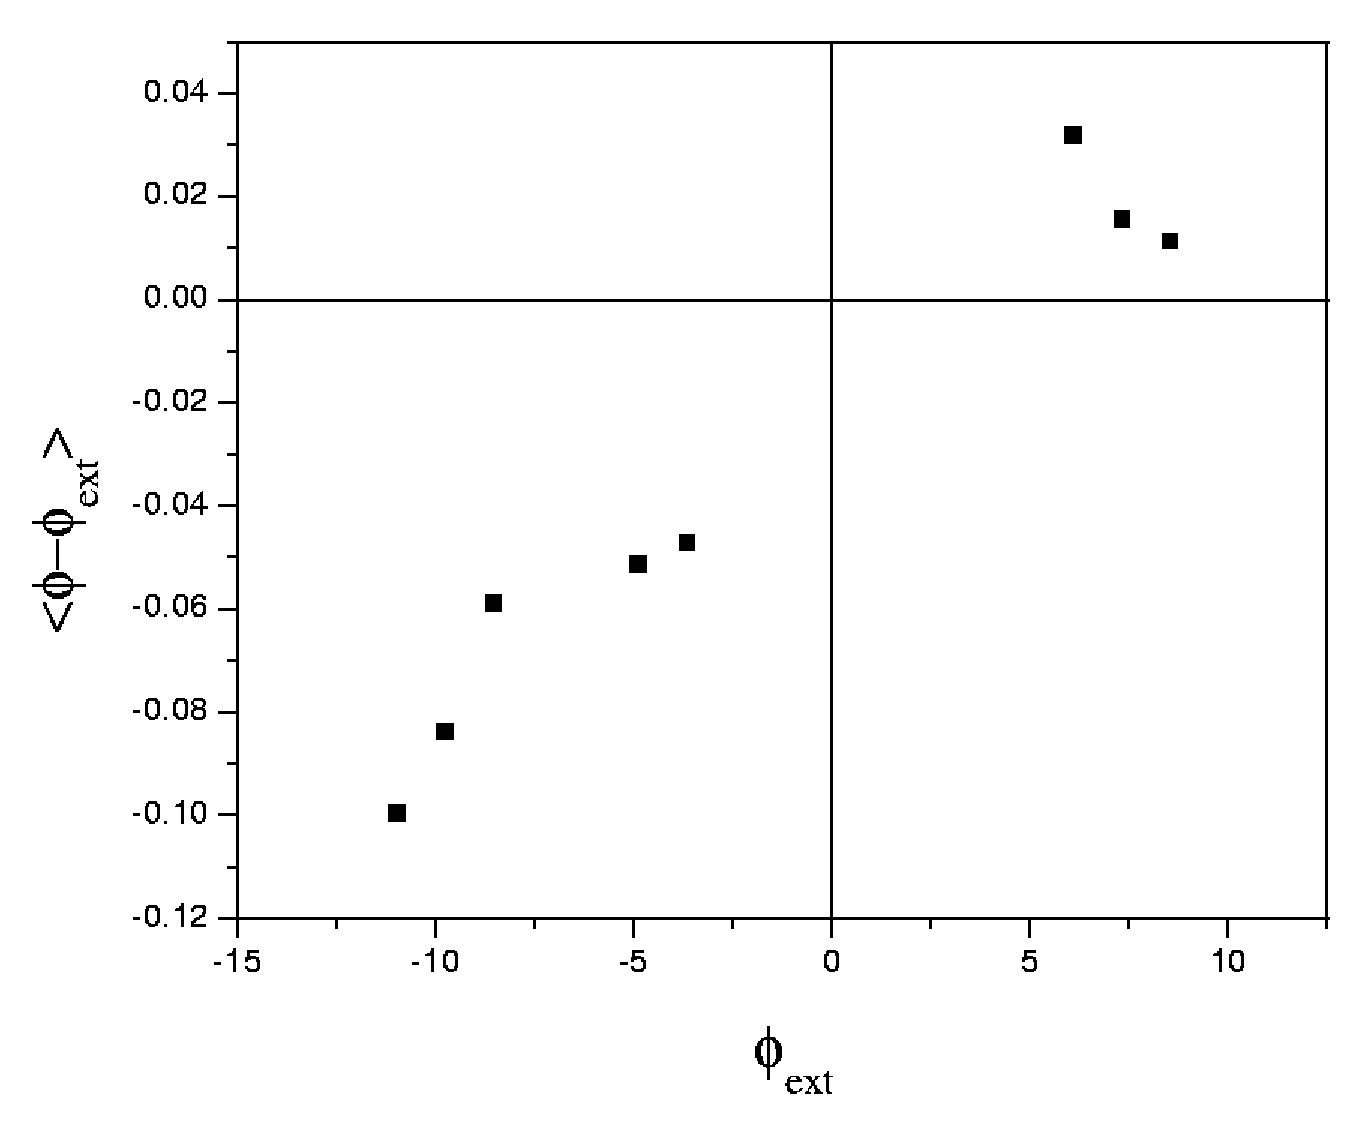
\includegraphics[width=5.7in]{figs/pme_exp/fig3_10.eps}
\caption[Measured mean magnetization versus cooling field for
$100 \times 150$ junction array.]{Measured mean magnetization versus
cooling field for the $100 \times 150$ \jja. The error for each 
data point is smaller than the size of the symbol.}
\label{fig:lg_mag_vs_ext}
\end{figure}

\section{Summary of magnetization measurements}

Arrays of $30 \times 100$ and $100\times 150$ junctions were
measured in field-cooling experiments using a scanning SQUID microscope. 
The results on the arrays are very similar, both in magnitude of 
array magnetization and in average 
magnetization dependence upon external field. 
The next chapter will explain the various phenomena observed
here and reconcile them with the ideas presented in 
chapter \ref{chap:jjarray}. 

In both cases the array magnetization increases with increasing external
field, and the array is preferentially paramagnetic. This is in contrast
to the single-loop model which predicts equally that the the single loop
will be either paramagnetic or diamagnetic equally often.  

The magnetization internal to the array takes on a somewhat complicated,
randomly distributed arrangement. The magnetization
at the edge is always diamagnetic, regardless of the internal magnetization. 

 
